\documentclass[12pt]{article}
%Had an issue with too many packages so needed to put this in to work around it.
\usepackage{etex}

\usepackage{amssymb,amsmath,amsthm,mathtools}
\usepackage{hyperref,cleveref}
\usepackage[margin=1.25in]{geometry}
\usepackage{graphicx,ctable,booktabs} 
\usepackage[parfill]{parskip} % begin paragraphs on empty line rather than indent
\usepackage{fancybox}
\usepackage{tipa} % for \textpipe
\usepackage{caption}
\usepackage{subcaption}
\usepackage{bbm}


\usepackage{tikz}
\usetikzlibrary{shapes,arrows,positioning}

\usepackage{epstopdf} % eps to pdf, declare graphics
\usepackage{soul} % enable highlighting text: use \hl{your text here}
\DeclareGraphicsRule{.tif}{png}{.png}{`convert #1 `dirname #1`/`basename #1 .tif`.png}
\def\thesection{\arabic{section}} % adjust section and subsection labelling 
\def\thesubsection{\arabic{section}(\alph{subsection})}
\makeatletter
\newenvironment{pr}{\@startsection % section as pr
       {section}{1}
       {0.4em}{-.5ex plus -1ex minus -.2ex}{.5ex plus .2ex}
       {\pagebreak[3]\large\bf\noindent{Problem}}}
       {\nopagebreak[3]\vspace{3ex}}
\newenvironment{pa}{\@startsection % subsection as pa
       {subsection}{2}
       {0.3em}{0ex plus -1ex minus -.2ex}{.5ex plus .2ex}
       {\pagebreak[3]\large\noindent{}}}
       {\nopagebreak[3]\vspace{3ex}}
\makeatother
\usepackage{fancyhdr}
\pagestyle{fancy}
\lhead{\footnotesize D.Deriso, N. Banerjee, A. Fallou} % header left
\chead{\footnotesize} % header center
\rhead{\thepage} % header right
\lfoot{} 
\cfoot{} 
\rfoot{} 
\renewcommand{\headrulewidth}{.3pt} 
\renewcommand{\footrulewidth}{.3pt}
\setlength\voffset{-0.25in}
\setlength\textheight{648pt}

\setlength{\tabcolsep}{8pt}

\setlength{\parindent}{1cm}
\renewcommand{\arraystretch}{1.2}
% big-O notation
\newcommand{\bigO}[1]{\ensuremath{\mathop{}\mathopen{}\mathcal{O}\mathopen{}\left(#1\right)}}
%%%%%%%%%%%%%%%%%%%%%%%%%%%%%%%

%%%%%%%%%%%%%%%%%%%%%%%%%%%%%%
% Code blocks formatting
\usepackage{listings}
\usepackage{color}

\definecolor{dkgreen}{rgb}{0,0.6,0}
\definecolor{gray}{rgb}{0.5,0.5,0.5}
\definecolor{mauve}{rgb}{0.58,0,0.82}

\lstset{frame=tb,
  language=matlab,
  aboveskip=3mm,
  belowskip=3mm,
  showstringspaces=false,
  columns=flexible,
  basicstyle={\scriptsize\ttfamily},
  numbers=none,
  numberstyle=\tiny\color{gray},
  keywordstyle=\color{blue},
  commentstyle=\color{dkgreen},
  stringstyle=\color{mauve},
  breaklines=true,
  breakatwhitespace=true,
  tabsize=3
}

\makeatletter
\newenvironment{CenteredBox}{% 
\begin{Sbox}}{% Save the content in a box
\end{Sbox}\centerline{\parbox{\wd\@Sbox}{\TheSbox}}}% And output it centered
\makeatother

%%%%%%%%%%%%%%%%%%%%%%%%%%%%%%
\begin{document}

  \title{CS 229 : Project progress report}
  \author{D.Deriso, N. Banerjee, A. Fallou}
  \date{\today}
  \maketitle
  \thispagestyle{empty}
  %%%%%%%%%%%%%%%%%%%%%%%%%%%%%%%



\section*{Introduction}
%
\small  
Cardiovascular health is the \emph{sin qua non} of human life. Early detection of cardiovascular disease is of paramount importance in public health. This project aims to develop a method to visualize the perfusion of blood through the skin via pulse oximetry. Pulse oximetry is a technique that exploits the fact that oxygenated and deoxygenated hemoglobin changes the color of red blood cells. The technique maps these changes in rgb color of the visible skin to the invisible presence of oxygenated vs deoxygenated blood in the local vasculature underneath the skin.

Previous studies have shown that video obtained from an ordinary webcam can be used to visualize perfusion by selectively amplifying temporal frequencies in video \footnote{http://people.csail.mit.edu/mrub/vidmag/}. A study by the MIT CSAIL showed that this technique can also be used to infer heart rate from the person being taped. The present project aims to extend this work to detect the relative changes in oxygenated vs deoxygenated blood and reconstruct the pulse oximeter waveform from an ordinary webcam video.



\section{Methods}

Previous work on Eulerian Video Magnification (EVM), has led to the following processing pipeline, which we later modify for our purpose. The video can undergo different treatments, but the central goal is to amplify spatial or temporal changes that are normally invisible to the naked eye. The process can be summarized as:

\begin{itemize}
\item Separate the video into distinct spatial frequency bands by performing a 2D spatial fourier decomposition. 
\item For each spatial frequency band, blur and downsample several times using Gaussian or Laplacian Pyramids. The first step preserves spatial features (e.g. high frequencies such as edges) through this destructive process.
\item Amplify a pre-selected temporal frequency band.
\item Recombine spatial frequencies from step 1, and add the amplified video to the original video.
\end{itemize}
Figure 1 presents an example for the output of the next-to-last-step. 

\begin{figure}
\begin{subfigure}{.5\textwidth}
\captionsetup{justification=centering}
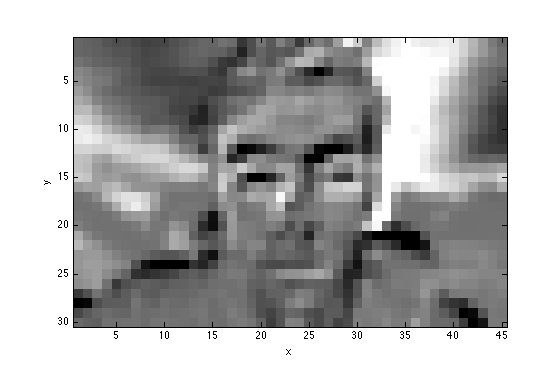
\includegraphics[width=\textwidth]{images/red_peak.png}
\caption{At at a given time}
\end{subfigure}
\begin{subfigure}{.5\textwidth}
\captionsetup{justification=centering}
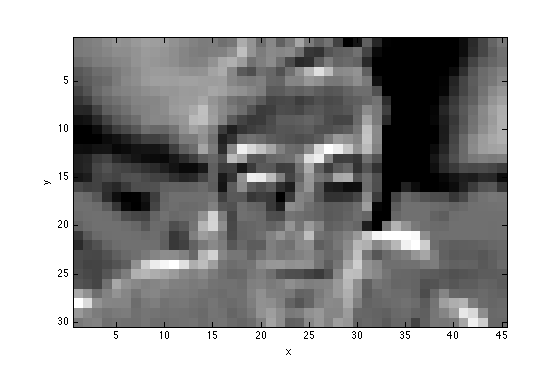
\includegraphics[width=\textwidth]{images/red_trough.png}
\caption{Half a heartbeat period later}
\end{subfigure}
\captionsetup{justification=centering}
\caption{Red channel of the EVM output, before recombining with the original video.}
\end{figure}

Strikingly, these two frames showed that the whole video undergoes a periodic color change with a frequency that seems equal to the heartbeat. This did not happen with the data provided in the paper, where in a similar video only the person's face changes color.
To extract features relevant to pulse oximetery, we seek out a weighted combination of periodic changes in color space that best reconstruct our training pulse oximetery signal. We therefore undergo the following process:

\begin{itemize}
\item Extract each pixel’s time course from the video. 
\item For each pixel, separate the colors into R, G, B bands and perform a fourier decomposition where frequency is grouped into n bins.
\item Learn weights via linear regression for frequencies within each color band to reproduce the simultaneously recorded pulse oximeter data in the training data set. 
\item Amplify the temporal frequencies according to the weights of the regression.
\item Combine the amplified video with the original video.
\end{itemize}


  


\section{Model}
  This new understanding of our problems naturally means that our core set of predictors are the three color channel intensity values through
  time \(I_R(t), I_G(t), I_B(t)\), which are infinite-dimensional feature vectors, and we want to do a regression of the reading of our pulse oximeter $Ox(t)$ 
  on these intensity values.
  We then made two additional prior assumptions:
  \begin{itemize}
    \item We are only interested in periodic phenomena.
    \item These phenomena have a frequency lying in the 0-5Hz range.
  \end{itemize}

  The first assumption means we can take Fourier series decomposition of our intensity/oximetry values, the second that we can
  limit the decomposition to only a small number $p$ of harmonics. We took $p$ = 10 as a starting value:
  \[
    I(t)/Ox(t) = \sum_{n=-p}^{p} c_n e^{i \left(\frac{2\pi nt}{T}  + \phi_n \right) }
  \]

  Thus, our training output $y$ is a vector of size $2p$, with the coefficients of the Fourier decomposition.
  Our feature vector contains the $2p$ coefficients of the Fourier decomposition for each of the three color channels.
  Each pixel is considered a different training example, we have $k$ of them for one video (typically \(k=1280\times 720\)).
  Thus our parameters matrix, $\theta \in \mathbb{R}^{(6p) \times k}$


\section{Initial results}
  Our initial computations on the pixel-intensity data revealed, unsurprisingly,
  that pixel intensity variation over time for a reasonably still video was not large.
  Often a single color channel for a pixel would have a range of 3 (when it could vary from 0-255) over the whole video, even if that pixel was contained in the face.
  The DFT of the data would produce large peaks at 0 Hz and would rapidly diminish in magnitude. Because of this, we have not had any significant linear regression results.
  A simple solution is to subtract a mean intensity value of our pixel, so as to increase the relative intensity variations over time.
  Ultimately, we may have to resort to using EVM-enhanced videos if our training data has signals that are too weak to pick up.
  
    %%%%%%%%%%%%%%%%%%%%%%%%%%%%%%%
  \end{document}
  
  